\documentclass{article}
\usepackage{microtype,graphicx,booktabs,amsmath,amssymb,hyperref}
\newcommand{\theHalgorithm}{\arabic{algorithm}}
\usepackage{icml2021}
\icmltitlerunning{Beyond Polynomial Expansion: Revisiting Kryptonite-3.0}
\begin{document}
\setcounter{dbltopnumber}{1}
\raggedbottom
\twocolumn[
\icmltitle{Beyond Polynomial Expansion: Revisiting Kryptonite-3.0 Through Representation, Data Scaling, and Low-Rank Adaptation}
\begin{icmlauthorlist}
\icmlauthor{Charlie Wang, Zihao Zhao, Jerry Li, William Chia}{imp}
\end{icmlauthorlist}
\icmlaffiliation{imp}{Imperial College London, London, United Kingdom}
\icmlcorrespondingauthor{Coursework team}{No email given}
\vskip 0.3in
]
\printAffiliationsAndNotice{}
\footnotetext{Development repository: \url{https://github.com/jerryliruijie/Kryptonite_v3.0}. Submission GitLab URL and final reproducible commit remain to be supplied.}

\begin{abstract}
Challenge datasets can reveal the limitations of machine learning methods, but poor performance from a restricted set of models does not necessarily imply that a task is unlearnable. Kryptonite-3.0 draws broad conclusions from the failure of polynomial classifiers, limited benefits from additional training data, and unsuccessful transfer of pretrained representations. In this work, we revisit these claims by investigating alternative classifiers and input representations, the effects of training-set size, and low-rank adaptation (LoRA) of KryptoNet-40. On Kryptonite-20, -30, and -40, sign-CatBoost achieves 93.44–96.28\% local-test accuracy, compared with 53.41–54.50\% for quadratic logistic regression. An MLP trained from scratch also exceeds 90\% accuracy on all three datasets. Matched learning curves further show that additional training data yields substantially greater improvements for sign-CatBoost than for the quadratic baseline. On Kryptonite-40-Adapt, LoRA achieves 95.75–96.00\% mean local-test accuracy across the evaluated ranks, with rank-1 adaptation training only 0.51\% of the model's parameters. Together, these findings demonstrate that the failures reported in Kryptonite-3.0 do not generalize to the alternative learning approaches evaluated in this study.
\end{abstract}

\section{Introduction}
Challenge datasets play an important role in evaluating the capabilities and limitations of machine learning models. However, poor performance on a particular benchmark does not necessarily indicate a fundamental limitation of machine learning. In practice, a model's performance depends on its expressive capacity, the effectiveness of optimization, and its ability to generalize to unseen data. Although universal approximation theorems establish that certain neural networks can approximate a broad class of functions, they do not guarantee successful training or generalization with finite data (Leshno et al., 1993). Consequently, the failure of a particular learning method does not imply that a task is inherently unsolvable.

Kryptonite-3.0 (Quinn and Luther, 2026) challenges the effectiveness of machine learning through three main findings. First, polynomial logistic regression achieves less than 59\% accuracy even with polynomial features of degree 10, which the authors interpret as evidence against universal approximation. Second, quadrupling the training data produces only marginal improvements in quadratic logistic regression, leading the authors to question whether additional data can solve these tasks. Third, despite achieving 95\% accuracy on its pretraining task, KryptoNet-40 performs poorly under zero-shot evaluation and frozen-representation probing. However, these experiments examine a limited range of models and adaptation strategies. In particular, the failure of frozen representations does not establish whether updating the pretrained network could improve downstream performance.

To address these limitations, we systematically investigate alternative classification methods, the effects of training-set size, and parameter-efficient adaptation. We first compare logistic regression baselines with gradient-boosted decision trees and multilayer perceptrons (MLPs) trained from scratch. We combine a sign-based input representation with CatBoost to classify the three main Kryptonite datasets. We then investigate the relationship between training-set size and generalization by comparing learning curves on identical training subsets. Finally, we apply low-rank adaptation (LoRA) to KryptoNet-40, allowing its internal representations to be updated while keeping the pretrained hidden weights frozen.

Our main contributions are threefold:

\begin{enumerate}
\item \textbf{Representation-aware classification.} We demonstrate that both sign-transformed CatBoost and MLPs trained from scratch exceed 90\% local-test accuracy across all three main Kryptonite datasets. Furthermore, we show that the effectiveness of sign-based representations depends on the classifier.
\item \textbf{Model-dependent data scaling.} Matched learning curves show larger gains from increasing the training data for sign-transformed CatBoost than for quadratic logistic regression.
\item \textbf{Parameter-efficient adaptation.} We demonstrate that LoRA enables effective adaptation of KryptoNet-40, achieving over 95\% mean local test accuracy across the evaluated ranks. We also provide a mathematical analysis of its trainable parameter count and computational complexity relative to full fine-tuning.
\end{enumerate}

\section{Methodology}
\subsection{Classification objective and polynomial controls}
For labelled observations $\mathcal D=\{(x_j,y_j)\}_{j=1}^m$, with $x_j\in\mathbb R^d$ and $y_j\in\{0,1\}$, a model produces a logit $z_\theta(x)$ and probability $p_\theta(x)=\sigma(z_\theta(x))$, where $\sigma(z)=(1+e^{-z})^{-1}$. We minimize binary cross-entropy,
\begin{equation}
\mathcal L=-\frac1m\sum_{j=1}^m\left[y_j\log p_j+(1-y_j)\log(1-p_j)\right].
\label{eq:bce}
\end{equation}
Logistic regression uses $z_\theta(x)=w^\top\phi(x)+b$. The linear control sets $\phi(x)=x$; the quadratic control includes the original coordinates and all products $x_i x_k$ for $i\leq k$. Its feature dimension is $d+d(d+1)/2$, excluding the intercept. Both use L2-regularized log loss, inverse regularization strength $C=0.85$, and L-BFGS with at most 1,000 iterations and tolerance $10^{-6}$. A training-majority classifier checks the approximately balanced task. The controls use the shared split; Kryptonite-3.0 evaluates a normalized degree-1--10 kernel.

\subsection{Sign-based CatBoost}
We use a binary representation of each input feature based on its sign. Sign-based binary representations have been studied for classification \cite{needell2018}. The starter implementation accompanying Kryptonite-3.0 also applies a sign transformation before its polynomial kernel \cite{quinn2026}. We combine sign-transformed inputs with CatBoost to learn interactions between feature signs. For an input $x\in\mathbb R^d$, we set
\begin{equation}
s_i(x)=\begin{cases}+1,&x_i\geq0,\\-1,&x_i<0.\end{cases}
\label{eq:sign}
\end{equation}
CatBoost \cite{prokhorenkova2018} combines decision trees in an additive model. Given the sign-transformed input, the logit and predicted probability are
\begin{align}
F_t(s)&=F_{t-1}(s)+\eta T_t(s),\nonumber\\
p(x)&=\sigma(F_T(s(x))).
\end{align}
Here $T_t$ is the tree added at iteration $t$ and $\eta$ controls its contribution. Let $\ell_j$ be the per-example binary cross-entropy in Equation~\ref{eq:bce} and $p_{j,t-1}=\sigma(F_{t-1}(s(x_j)))$. Its negative gradient with respect to the current logit is
\begin{equation}
-\frac{\partial\ell_j}{\partial F_{t-1}(s(x_j))}=y_j-p_{j,t-1}.
\end{equation}
CatBoost uses gradient information to construct each tree and estimate its leaf values. Each symmetric tree applies the same split at a given depth. A path through the tree combines conditions on the signs of features, and its leaf value contributes to the logit. We use 600 symmetric trees of depth 10, a learning rate $\eta=0.05$, and leaf L2 regularization 10. A depth-10 tree has at most $2^{10}=1024$ leaves. The final prediction is class 1 when $p(x)>0.5$ and class 0 otherwise.

\subsection{MLPs and optimization}
The scratch MLP uses two ReLU hidden layers of equal width $h\in\{128,256\}$:
\begin{align}
h_1&=\operatorname{ReLU}(W_1\tilde x+b_1),\nonumber\\
h_2&=\operatorname{ReLU}(W_2h_1+b_2),\qquad z=w^\top h_2+b.
\end{align}
Here $\tilde x_i=(x_i-\mu_i)/\sigma_i$, with statistics fitted only on training rows. The model retains continuous magnitudes and learns a nonlinear representation, providing a complementary test to sign-based trees.

Adam \cite{kingma2015} uses gradient $g_t$, moment estimates $u_t=\beta_1u_{t-1}+(1-\beta_1)g_t$ and $v_t=\beta_2v_{t-1}+(1-\beta_2)g_t^2$, and the elementwise update
\begin{align}
\hat u_t&=\frac{u_t}{1-\beta_1^t},\qquad \hat v_t=\frac{v_t}{1-\beta_2^t},\nonumber\\
\theta_{t+1}&=\theta_t-\eta\frac{\hat u_t}{\sqrt{\hat v_t}+\epsilon}.
\end{align}
We use $(\beta_1,\beta_2)=(0.9,0.999)$, $\epsilon=10^{-8}$, $\eta=10^{-3}$ and batch size 256. Coupled weight decay adds $10^{-4}\theta_t$ to the loss gradient. During initial development, training ran for at most 150 epochs, with a minimum of 30 and patience 20 for validation-accuracy improvement. The checkpoint maximized validation accuracy, with lower validation loss breaking ties.

\subsection{Low-rank adaptation of KryptoNet-40}
KryptoNet-40 has four width-512 ReLU hidden layers and a scalar output head, totalling 809,473 parameters. For a pretrained layer $W\in\mathbb R^{o\times i}$, LoRA \cite{hu2022} computes
\begin{equation}
Y=WX+b\mathbf1^\top+sBAX,\qquad s=\alpha/r,
\label{eq:lora}
\end{equation}
where $X\in\mathbb R^{i\times N}$, $A\in\mathbb R^{r\times i}$ and $B\in\mathbb R^{o\times r}$. We freeze $W,b$, initialize $A$ with Kaiming-uniform values and $B$ to zero, and train $A,B$. Thus the initial layer equals its pretrained counterpart, while $\operatorname{rank}(BA)\leq r$ constrains the update. The rank sets the width of the bottleneck through which the update acts: $AX$ projects each input onto $r$ directions, and $B$ maps them back to the output space. Thus $r$ controls both the update's capacity and its $r(i+o)$ trainable parameters, and a small $r$ acts as a regularizer. We fix $\alpha=8$ for every rank, so $s=8/r$. We adapt all four hidden layers and train the existing output head, using raw inputs.

LoRA and the linear probe use Adam with the default $\beta$ and $\epsilon$ of Section~2.3, no weight decay and batch size 128. The learning rate is $10^{-3}$ for LoRA and $10^{-2}$ for the probe, whose head is reinitialized. During initial development, training used at most 300 epochs and patience 40. The checkpoint maximized validation accuracy, with lower validation loss breaking ties; an improvement of either kind reset the patience counter.

Writing $Z=AX$ and $G=\partial\mathcal L/\partial Y$, backpropagation gives
\begin{align}
\nabla_B\mathcal L&=sGZ^\top,& G_Z&=sB^\top G,\nonumber\\
\nabla_A\mathcal L&=G_ZX^\top,&\nabla_X\mathcal L&=W^\top G+A^\top G_Z.
\label{eq:gradients}
\end{align}
Initially $\nabla_A\mathcal L=0$, but $B$ can receive a nonzero gradient. Freezing $W$ removes its parameter gradient, while $W^\top G$ propagates gradients to earlier trainable layers.

\subsection{Training-step operation counts}
We count an $n\times m$ by $m\times k$ product as $nmk$ operations. One step means a forward and backward pass over $N$ inputs; bias additions, nonlinearities, scalar operations and optimizer updates are excluded. Full fine-tuning trains $oi+o$ parameters, including bias, and costs $3oiN$ if an input gradient is needed: $WX$, $GX^\top$ and $W^\top G$.

Evaluating $B(AX)$ and caching $Z$ costs $oiN+rN(i+o)$ forward operations. The parameter and intermediate gradients in Equation~\ref{eq:gradients} cost $rN(i+2o)$, and the input gradient costs $oiN+irN$. Consequently,
\begin{equation}
C_{\mathrm{LoRA}}=2oiN+3rN(i+o),\qquad
P_{\mathrm{LoRA}}=r(i+o).
\label{eq:cost}
\end{equation}
If the input gradient is unnecessary, the full and LoRA costs become $2oiN$ and $oiN+rN(2i+3o)$, respectively. The latter applies to the first hidden layer when the input data require no gradient.

Product order matters in both passes. Forming $(BA)X$ costs $oir+oiN$ for the update alone, instead of $rN(i+o)$ for $B(AX)$. Similarly, computing $\nabla_A\mathcal L$ as $s(B^\top G)X^\top$ costs $rN(o+i)$, whereas $sB^\top(GX^\top)$ costs $oiN+roi$. Reusing $Z$ in $GZ^\top$ also avoids a dense intermediate. Efficient order depends on the dimensions and cached products; the factored order is appropriate for our small ranks.

Including the trainable 513-parameter head, the network has $3624r+513$ trainable parameters. Applying the appropriate first-layer count and including all later layers gives
\begin{align}
C_{\mathrm{full,net}}&=2{,}401{,}792N,\nonumber\\
C_{\mathrm{LoRA,net}}&=(1{,}594{,}880+10{,}832r)N.
\label{eq:networkcost}
\end{align}
At $r=1$, LoRA trains 0.51\% of parameters and uses 66.85\% of full fine-tuning's matrix operations per training step. For $N=128$, these counts match half of PyTorch's FLOP counter, which counts multiplication and addition separately, for full fine-tuning and for $r\in\{1,2,4,8\}$.

\begin{figure*}[t]
\centering
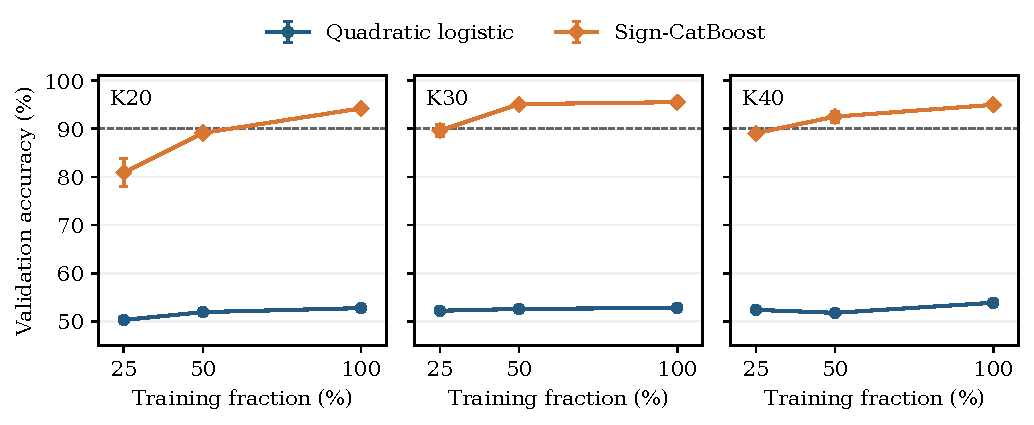
\includegraphics[width=\textwidth]{figures/learning_curves_3seed_layout.pdf}
\caption{Validation accuracy on matched nested training subsets. Both methods use the same rows at each fraction and the same fixed validation set. Full training sizes are 8,400, 14,000 and 22,400 for K20, K30 and K40. Points and error bars show mean and sample standard deviation over three model seeds on the same split. Quadratic logistic regression is deterministic. Lines guide the eye; the dashed line marks 90\%.}
\label{fig:scaling}
\end{figure*}

\section{Experimental Design}
\subsection{Partitions and evaluation roles}
We use the supplied labelled datasets and shared stratified 70/20/10 train/validation/local-test partitions, with split seed 67 (Table~\ref{tab:data}). Initial development used the 70\% training partition and the 20\% validation partition. We then refitted candidate models using their combined 90\% and evaluated them on the held-out 10\%. Data-dependent preprocessing was fitted on the 90\% training rows only. The local-test results were inspected during development and used to select final methods and rank, so the resulting scores describe test-selected models. Classification accuracy is the primary metric; the original paper's 90\% target provides a reference.



\begin{table}[t]
\centering
\caption{Shared labelled-data partitions. The adaptation task has 40 input dimensions. Each separate hidden set has 10,000 unlabelled examples.}
\begin{tabular}{lrrr}\toprule
Dataset & Train & Validation & Local test \\\midrule
K20 & 8,400 & 2,400 & 1,200 \\
K30 & 14,000 & 4,000 & 2,000 \\
K40 & 22,400 & 6,400 & 3,200 \\
K40-Adapt & 2,800 & 800 & 400 \\\bottomrule
\end{tabular}
\label{tab:data}
\end{table}

For the local-test comparisons in Tables~\ref{tab:main} and~\ref{tab:adapt}, majority classification, logistic regression and sign-CatBoost were fitted on the combined 90\% training and validation rows. The MLP, linear probe and LoRA were trained on the 70\% training rows, with their best checkpoints selected on the fixed 20\% validation rows; these models were not refitted on the combined 90\%. All methods were evaluated on the same fixed 10\% local-test partition for their dataset. The stochastic methods use training seeds 42, 123 and 2026 on a macOS arm64 CPU with one numerical training thread. The selected MLP width is 256, and LoRA rank 1 has the highest mean validation accuracy among the evaluated ranks. The MLP and adaptation models predict class 1 when the logit exceeds zero. Table entries report mean local-test accuracy and sample standard deviation across the three seeds; majority classification, L-BFGS logistic regression and zero-shot inference are deterministic here.

\subsection{Hypotheses and controlled comparisons}
\textbf{H1: Alternative learning methods can overcome the limitations of polynomial classifiers.} Kryptonite-3.0 reports that polynomial logistic regression fails to reach its 90\% accuracy target, even with high-degree feature expansion. We investigate whether this limitation extends to other learning approaches by comparing majority, linear and quadratic logistic baselines with sign-transformed CatBoost and MLPs trained from scratch. Sign-based CatBoost tests a binary feature representation combined with gradient-boosted trees.

\textbf{H2: The benefits of additional training data depend on the learning procedure.} Kryptonite-3.0 observes only marginal improvements when increasing the training data for quadratic logistic regression. To examine whether this finding generalizes, we compare its learning curve with that of sign-transformed CatBoost. Both methods are trained on identical nested subsets containing 25\%, 50\%, and 100\% of the available training data and evaluated on the same validation set, with hyperparameters fixed across training sizes. The subsets use seed 42. This comparison evaluates complete learning procedures, including model architecture and input representation.

\textbf{H3: LoRA can improve KryptoNet-40 adaptation beyond frozen-representation baselines.} Kryptonite-3.0 reports poor performance from zero-shot inference and frozen-feature probing, leaving adaptation of the pretrained hidden layers unexplored. We investigate whether updating these representations can improve downstream performance by comparing zero-shot KryptoNet-40, linear probing, and LoRA with ranks $(r\in\{1,2,4,8\})$ on Kryptonite-40-Adapt. Each trainable configuration is evaluated across three random seeds. LoRA adapts the hidden layers while retaining and training the pretrained output head, whereas the linear probe reinitializes its head and keeps the hidden layers frozen.





\begin{table*}[t]
\centering
\caption{Local-test accuracy (\%) on one fixed split. Majority, logistic regression and sign-CatBoost use the combined 90\% training and validation rows; the MLP uses the 70\% training rows and a validation-selected checkpoint. Entries are mean $\pm$ sample standard deviation across seeds 42, 123 and 2026. Majority and L-BFGS logistic regression are deterministic, with identical repetitions.}
\begin{tabular}{lrrr}\toprule
Method & K20 & K30 & K40 \\\midrule
Majority & $50.42 \pm 0.00$ & $50.05 \pm 0.00$ & $50.19 \pm 0.00$ \\
Linear logistic & $49.58 \pm 0.00$ & $48.95 \pm 0.00$ & $48.84 \pm 0.00$ \\
Quadratic logistic & $53.92 \pm 0.00$ & $54.50 \pm 0.00$ & $53.41 \pm 0.00$ \\
Sign-CatBoost & $93.44 \pm 0.05$ & $96.28 \pm 0.25$ & $96.24 \pm 0.05$ \\
MLP (width 256) & $89.42 \pm 0.80$ & $91.87 \pm 0.63$ & $93.64 \pm 0.69$ \\
\bottomrule
\end{tabular}
\label{tab:main}
\end{table*}

\begin{figure*}[t]
\centering
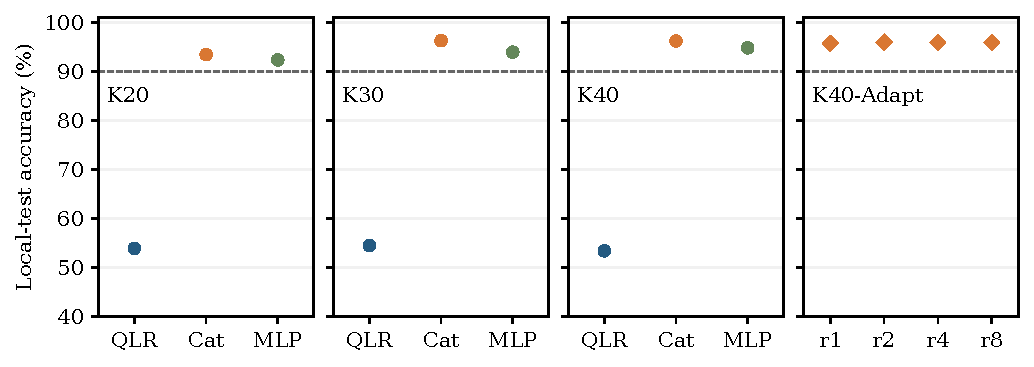
\includegraphics[width=\textwidth]{figures/test_3seed_layout.pdf}
\caption{Local-test accuracy after refitting on the combined training and validation partitions. Quadratic logistic regression, sign-CatBoost and the MLP are shown for K20, K30 and K40; the right panel shows LoRA ranks on K40-Adapt. Points and error bars show mean and sample standard deviation over three seeds on one split. The dashed line marks 90\%.}
\label{fig:refit}
\end{figure*}

\begin{table}[t]
\centering
\caption{K40-Adapt local-test accuracy on 400 examples, reported as mean $\pm$ sample standard deviation across seeds 42, 123 and 2026. The linear probe and LoRA use 2,800 training rows and checkpoints selected on 800 validation rows. Zero-shot is deterministic; its repeated predictions are identical.}
\begin{tabular}{lrr}\toprule
Method & Trainable params & Accuracy (\%) \\\midrule
Zero-shot & 0 & $49.00 \pm 0.00$ \\
Linear probe & 513 & $49.50 \pm 0.43$ \\
LoRA $r=1$ & 4,137 & $95.58 \pm 0.14$ \\
LoRA $r=2$ & 7,761 & $94.75 \pm 1.32$ \\
LoRA $r=4$ & 15,009 & $95.83 \pm 0.29$ \\
LoRA $r=8$ & 29,505 & $95.67 \pm 0.14$ \\
\bottomrule
\end{tabular}
\label{tab:adapt}
\end{table}

\section{Experimental Results}
\subsection{Alternative classifiers exceed the polynomial controls}
Sign-CatBoost achieves mean local-test accuracies of 93.44\%, 96.28\%, and 96.24\% on Kryptonite-20, -30, and -40, respectively (Table~\ref{tab:main}). Its class-1 F1 means are 93.37\%, 96.30\%, and 96.24\%. Quadratic logistic regression achieves 53.83\%, 54.50\%, and 53.44\% accuracy on the same sets. CatBoost is selected for each hidden prediction set using these local-test comparisons.




The MLP uses standardized continuous inputs and achieves mean local-test accuracies of 92.22\%, 93.67\%, and 94.70\% on Kryptonite-20, -30, and -40, respectively.

\subsection{Matched learning curves}
Figure~\ref{fig:scaling} shows differences between the learning curves of the two methods. Mean sign-CatBoost validation accuracy increases across the three training sizes on each dataset. At 50\% of the original training partition, its mean accuracy is 89.44\%, 95.12\%, and 92.55\% for \mbox{K20, K30, and K40, respectively.} The quadratic baseline gains at most 2.71 percentage points from the smallest to the largest subset.

\subsection{LoRA permits adaptation with few trainable parameters}
On the Kryptonite-40-Adapt local test set, LoRA ranks 1, 4 and 8 achieve mean accuracies of at least 95.75\%, while rank 2 achieves 88.75\% (Table~\ref{tab:adapt}). Zero-shot inference and the refitted linear probe achieve 49.00\% and 48.33\%, respectively. Ranks 4 and 8 tie at a mean of 96.00\%; the prespecified tie-break selects the smaller rank, 4, for hidden prediction. Figure~\ref{fig:refit} shows the local-test comparisons across all four datasets.



Rank-4 LoRA trains 15,009 parameters, approximately 1.85\% of the network. Rank 2 ranges from 74.75\% to 96.00\% local-test accuracy across seeds under the fixed 13-epoch schedule. At epoch 13, training loss is 0.5454 for seed 2026 and 0.1492 for seed 123. The fixed $\alpha=8$ changes the scaling $s=8/r$ across ranks. Hidden predictions use single seed-42 checkpoints for the selected methods. The selected rank-4 checkpoint achieves 95.75\% local-test accuracy.



\section{Discussion}
\subsection{Revisiting Kryptonite-3.0's inferences}
Sign-CatBoost and the MLP achieve over 90\% local-test accuracy on all three main Kryptonite datasets. The matched curves show that the benefit of additional training data depends on the learning procedure. LoRA adapts KryptoNet-40 to Kryptonite-40-Adapt using low-rank updates to its hidden layers and a trainable output head.

Universal approximation establishes an existence result for a sufficiently rich function family under stated assumptions \cite{leshno1993}. A fitted model's accuracy also depends on the chosen model class, optimization, regularization and available training data.

\subsection{Further experiments}
Repeated outer splits would characterize performance across data partitions. Matched head-initialization, learning-rate and layer-placement experiments would further compare adaptation strategies.

\newpage
\subsection{Environmental impact}
The fresh experiments were run on a macOS arm64 CPU without a GPU; CatBoost and PyTorch training used one numerical thread. Run-level fitting times are recorded with the experiment outputs. The validation-selected rank-1 LoRA configuration trains 0.51\% of KryptoNet-40's parameters and uses 66.85\% of full fine-tuning's counted matrix operations per training step (Section~2.5). These operation counts do not directly measure energy use; no hardware power measurements were collected.

\begin{samepage}
\subsection{Conclusion}
Sign-CatBoost and the MLP achieve over 90\% local-test accuracy across Kryptonite-20, -30 and -40. The matched learning curves demonstrate model-dependent benefits from additional training data. Rank-4 LoRA adapts KryptoNet-40 to Kryptonite-40-Adapt with 96.00\% mean local-test accuracy while training 1.85\% of its parameters.

\end{samepage}

\begin{thebibliography}{9}
\bibitem[Hu et al.(2022)]{hu2022}
Hu, E. J., Shen, Y., Wallis, P., Allen-Zhu, Z., Li, Y., Wang, S., Wang, L., \& Chen, W. (2022).
LoRA: Low-rank adaptation of large language models.
In \emph{International Conference on Learning Representations}.
\url{https://arxiv.org/abs/2106.09685}.

\bibitem[Kingma \& Ba(2015)]{kingma2015}
Kingma, D. P., \& Ba, J. (2015).
Adam: A method for stochastic optimization.
In \emph{International Conference on Learning Representations}.
\url{https://arxiv.org/abs/1412.6980}.

\newpage
\bibitem[Leshno et al.(1993)]{leshno1993}
Leshno, M., Lin, V. Y., Pinkus, A., \& Schocken, S. (1993).
Multilayer feedforward networks with a nonpolynomial activation function can approximate any function.
\emph{Neural Networks}, \emph{6}(6), 861--867.
\url{https://doi.org/10.1016/S0893-6080(05)80131-5}.

\bibitem[Needell et al.(2018)]{needell2018}
Needell, D., Saab, R., \& Woolf, T. (2018).
Simple classification using binary data.
\emph{Journal of Machine Learning Research}, \emph{19}(61), 1--30.
\url{https://jmlr.org/papers/v19/17-383.html}.

\bibitem[Prokhorenkova et al.(2018)]{prokhorenkova2018}
Prokhorenkova, L., Gusev, G., Vorobev, A., Dorogush, A. V., \& Gulin, A. (2018).
CatBoost: Unbiased boosting with categorical features.
In \emph{Advances in Neural Information Processing Systems} (Vol. 31).
\href{https://proceedings.neurips.cc/paper/2018/hash/14491b756b3a51daac41c24863285549-Abstract.html}{NeurIPS 2018 proceedings}.

\bibitem[Quinn \& Luther(2026)]{quinn2026}
Quinn, H., \& Luther, L. (2026).
\emph{Kryptonite-3.0: The final end to machine learning hype?}
Mathematics for Machine Learning coursework mock paper, Imperial College London.
\end{thebibliography}
\end{document}